\usetikzlibrary{calc}
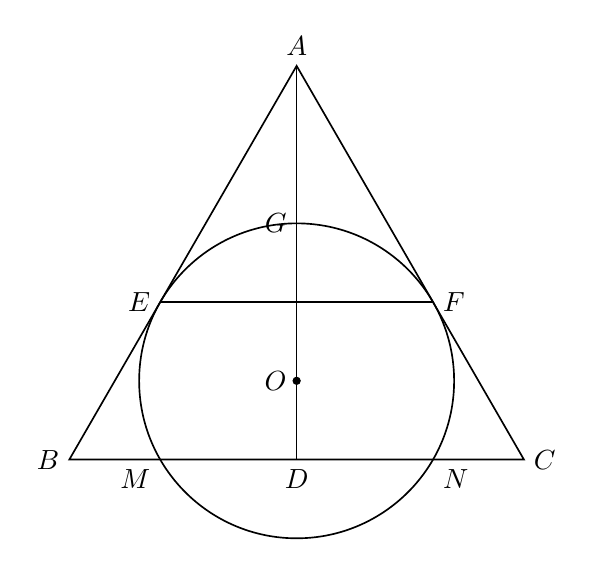
\begin{tikzpicture}[x=1cm,y=1cm,line width=.6pt,font=\normalsize]
\coordinate (O) at (0,0);
\coordinate (A) at (0,4);
\coordinate (G) at (0,2);
\coordinate (D) at (0,-1);
\coordinate (E) at (-1.73205,1);
\coordinate (F) at (1.73205,1);
\coordinate (M) at (-1.73205,-1);
\coordinate (N) at (1.73205,-1);
\coordinate (B) at (-2.88675,-1);
\coordinate (C) at (2.88675,-1);
\draw (O) circle[radius=2cm];
\draw (A)--(B)--(C)--cycle;
\draw (A)--(D);
\draw (E)--(F);
\draw (B)--(C);
\fill (O) circle (1.5pt);
\node[above] at (A) {$A$};
\node[left] at (G) {$G$};
\node[left] at (E) {$E$};
\node[right] at (F) {$F$};
\node[left] at (O) {$O$};
\node[left] at (B) {$B$};
\node[below left] at (M) {$M$};
\node[below] at (D) {$D$};
\node[below right] at (N) {$N$};
\node[right] at (C) {$C$};
\end{tikzpicture}
